% Options for packages loaded elsewhere
\PassOptionsToPackage{unicode}{hyperref}
\PassOptionsToPackage{hyphens}{url}
\PassOptionsToPackage{dvipsnames,svgnames*,x11names*}{xcolor}
%
\documentclass[
]{article}
\usepackage{amsmath,amssymb}
\usepackage{lmodern}
\usepackage{ifxetex,ifluatex}
\ifnum 0\ifxetex 1\fi\ifluatex 1\fi=0 % if pdftex
  \usepackage[T1]{fontenc}
  \usepackage[utf8]{inputenc}
  \usepackage{textcomp} % provide euro and other symbols
\else % if luatex or xetex
  \usepackage{unicode-math}
  \defaultfontfeatures{Scale=MatchLowercase}
  \defaultfontfeatures[\rmfamily]{Ligatures=TeX,Scale=1}
\fi
% Use upquote if available, for straight quotes in verbatim environments
\IfFileExists{upquote.sty}{\usepackage{upquote}}{}
\IfFileExists{microtype.sty}{% use microtype if available
  \usepackage[]{microtype}
  \UseMicrotypeSet[protrusion]{basicmath} % disable protrusion for tt fonts
}{}
\makeatletter
\@ifundefined{KOMAClassName}{% if non-KOMA class
  \IfFileExists{parskip.sty}{%
    \usepackage{parskip}
  }{% else
    \setlength{\parindent}{0pt}
    \setlength{\parskip}{6pt plus 2pt minus 1pt}}
}{% if KOMA class
  \KOMAoptions{parskip=half}}
\makeatother
\usepackage{xcolor}
\IfFileExists{xurl.sty}{\usepackage{xurl}}{} % add URL line breaks if available
\IfFileExists{bookmark.sty}{\usepackage{bookmark}}{\usepackage{hyperref}}
\hypersetup{
  pdftitle={Meeting3},
  pdfauthor={Kuan Liu},
  colorlinks=true,
  linkcolor=Maroon,
  filecolor=Maroon,
  citecolor=Blue,
  urlcolor=blue,
  pdfcreator={LaTeX via pandoc}}
\urlstyle{same} % disable monospaced font for URLs
\usepackage[margin=1in]{geometry}
\usepackage{graphicx}
\makeatletter
\def\maxwidth{\ifdim\Gin@nat@width>\linewidth\linewidth\else\Gin@nat@width\fi}
\def\maxheight{\ifdim\Gin@nat@height>\textheight\textheight\else\Gin@nat@height\fi}
\makeatother
% Scale images if necessary, so that they will not overflow the page
% margins by default, and it is still possible to overwrite the defaults
% using explicit options in \includegraphics[width, height, ...]{}
\setkeys{Gin}{width=\maxwidth,height=\maxheight,keepaspectratio}
% Set default figure placement to htbp
\makeatletter
\def\fps@figure{htbp}
\makeatother
\setlength{\emergencystretch}{3em} % prevent overfull lines
\providecommand{\tightlist}{%
  \setlength{\itemsep}{0pt}\setlength{\parskip}{0pt}}
\setcounter{secnumdepth}{-\maxdimen} % remove section numbering
\ifluatex
  \usepackage{selnolig}  % disable illegal ligatures
\fi

\title{Meeting3}
\author{Kuan Liu}
\date{Aug 17 2021}

\begin{document}
\maketitle

\hypertarget{chapter-4-phase-ii}{%
\section{Chapter 4 Phase II}\label{chapter-4-phase-ii}}

The primary objectives of Phase II study is to study efficacy. This
chapter focuses on Phase II adaptive design methods to evaluate
effectiveness, early stopping, and comparing efficacy between several
treatment arms.

\hypertarget{standard-design---frequentist}{%
\subsection{4.1 Standard Design -
frequentist}\label{standard-design---frequentist}}

\hypertarget{phase-iia}{%
\subsubsection{Phase IIA}\label{phase-iia}}

\begin{itemize}
\item
  to provide initial efficacy assessment, often designed single-arm,
  open label.
\item
  binary effective outcomes
\item
  two-stage optimal designs controlling type I and II errors
\item
  \begin{enumerate}
  \def\labelenumi{\alph{enumi})}
  \tightlist
  \item
    minimized expected sample size under null hypothesis (on the
    response rate)
  \end{enumerate}
\item
  \begin{enumerate}
  \def\labelenumi{\alph{enumi})}
  \setcounter{enumi}{1}
  \tightlist
  \item
    the minimax design, more conservative
  \end{enumerate}
\item
  multi-stage design with early stopping for futility, desireable but is
  more complicated to design comparing to two-stage
\end{itemize}

\hypertarget{phase-iib}{%
\subsubsection{Phase IIB}\label{phase-iib}}

\begin{itemize}
\tightlist
\item
  after IIA, a randomized and multi-arm study to select the ``winning''
  regimen.
\item
  time-to-event outcomes
\item
  larger type I and type II errors
\item
  optimal designs

  \begin{itemize}
  \item
    \begin{enumerate}
    \def\labelenumi{\alph{enumi})}
    \tightlist
    \item
      conventional design controlling type I\&II errors with emphasis on
      type II error
    \end{enumerate}
  \item
    \begin{enumerate}
    \def\labelenumi{\alph{enumi})}
    \setcounter{enumi}{1}
    \tightlist
    \item
      Pick-the Inner design (SWE), control only Type II error, ranking
      based design works best when there is a true ``winning'' regimen
    \end{enumerate}
  \end{itemize}
\item
  several limitations of these traditional frequentist based design.
  Flexible, adaptive Bayesian design is desired.
\end{itemize}

\hypertarget{predictive-probability-to-determine-effectiveness-and-early-stopping}{%
\subsection{4.2 Predictive probability to determine effectiveness and
early
stopping}\label{predictive-probability-to-determine-effectiveness-and-early-stopping}}

Example:

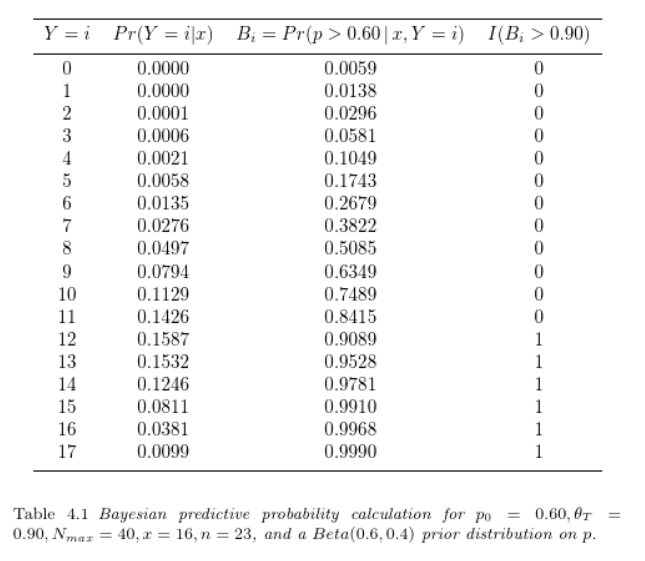
\includegraphics[width=0.8\textwidth,height=\textheight]{Table4.1.PNG}

\[PP=0.1587+0.1532+0.1246+0.0811+0.0381+0.0099=0.5656\]

For targeted \(\theta_L=0.10\) and \(\theta_U=0.9\), PP is between the
bounds which means the trial will not be stopped early (prior to 40 max
patients) for reasons of ineffective or effective.

\hypertarget{derivation-of-the-predictive-process-design}{%
\subsubsection{derivation of the predictive process
design}\label{derivation-of-the-predictive-process-design}}

\begin{itemize}
\item
  Given type I and type II error constraints, interim data and priors,
  find \(N_max\), \(\theta_L, \theta_T, \theta_U\).
\item
  Design with the smallest \(N_max\) but still achieve targeted response
  - similar conceptually to the minimax design
\item
  Allow investigator to monitor the trial
\item
  a minimum number of patients is required to gather reliable response
  rate before computing PP.
\end{itemize}

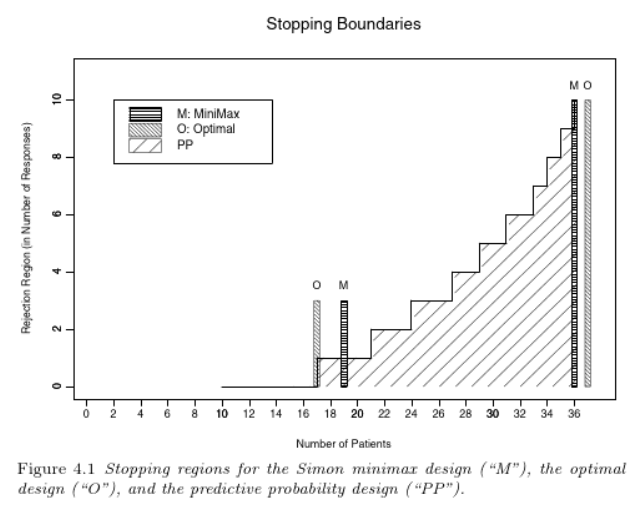
\includegraphics[width=0.8\textwidth,height=\textheight]{Figure4.1.PNG}

\hypertarget{sequential-stopping}{%
\subsection{4.2 Sequential stopping}\label{sequential-stopping}}

\begin{itemize}
\tightlist
\item
  Binary Stopping for futility and efficacy
\item
  Binary Stopping for futility and efficacy and toxicity
\end{itemize}

\hypertarget{adaptive-randomization-and-dose-allocation}{%
\subsection{4.3 Adaptive randomization and dose
allocation}\label{adaptive-randomization-and-dose-allocation}}

\begin{itemize}
\item
  ``Play with the winner'' over multiple rct for Phase IIB
\item
  Arms can be categorized into early loser (suspend), early winner,
  final winner and futility (immediate termination)
\item
  randomization probability is proportional to the posterior probability
  that an arm dominates another arm given the observed response rate of
  the two arms.
\item
  can select conservative prior or more liberal stopping rule (higher
  chance of finding early loser/winner) each will have different impact
  on the trial's operating characteristics
\item
  design can be prioritized based on number of patients to enrol,
  duration of the trial, small type I and II error.
\item
  adaptive randomization on treatment arm can also be used for dose
  finding
\item
  outcome adaptive randomization
\end{itemize}

R resources: - bayesCT package,
\href{https://cran.r-project.org/web/packages/bayesCT/vignettes/bayesCT.html}{An
R package for Simulation in Adaptive Bayesian Clinical Trials}

\end{document}
